\documentclass{article}

\usepackage[margin=2cm]{geometry}
\usepackage{graphicx}
\usepackage[utf8x]{inputenc}
\usepackage[english,russian]{babel}
\usepackage{blindtext}
\usepackage{tabularx}
\usepackage{rotating}
\usepackage{amssymb}
\usepackage{array}
\usepackage{vwcol}

\sloppy

\begin{document}
\hspace{0pt}
%\vfill
\begin{tabular}{p{0.3\textwidth}p{0.6\textwidth}}

\vspace{87}
\textbf{Ф617.}
\itshape Газетный текст фотографируется аппаратом «Зенит» c объективом, имеющим фокусное расстояние 50мм. дважды:\newline
1) c наименьшего допустимого для этого объектива a=0,5 м; \newline
2) после присоединения объектива к камере через удлинительное кольцо высотой h = 25 мм (таeже с минимально возможного расстояния). Найдите отношение размеров изображений, полученных на фотомплёнке в этих двух случаях.\newline 
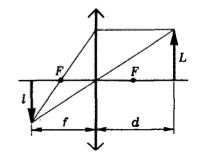
\includegraphics[width=0.29\textwidth]{image} 

&

\begin{center}
    Решая совместо уравнения (1) и (2), находим
\end{center}
\begin{center}
    $l_{1} = l \sqrt[3]{2}, d_{1} = d \sqrt[3]{4}$.
\end{center}
\begin{flushright}
    \itshapeИ. Слободецкий
\end{flushright}
\hspace{3}
\begin{rotate}{55}
    $\blacksquare$
\end{rotate}

Для решения задачи воспользуемся формулой линзы
\begin{center}
    $\frac{1}{d} + \frac{1}{f} = \frac{1}{F}$,
\end{center}
где d - рассотяние от фотографируемого предмета до объектива, f - расстояние от объектива до изображения, F - фокусное расстояние объектива (см. рисунок).\newline
При фотографировании текста в первом случае (без удлинительного кольца) $d_{1}=a$, и резкое изображение получается на расстоянии
\begin{center}
    $f_{1}=\frac{aF}{a-F}$.
\end{center}
Линейный размер изображения в этом случае равен (см. рисунок).
\begin{center}
    $l_{1} = L\frac{f_{1}}{a} = L\frac{F}{a-F}$.
\end{center}
\quad При присоединении объектива к камере через удлинительное колтцо высотой h резкое изображение текста получается на расстоянии
\begin{center}
    $f_{2}=f_{1}+h=\frac{aF}{a-F}+h$
\end{center}
от объектива. Минимально возможное расстояние от объектива, на котором может находиться при фотографировании текст, в этом случае равно
\begin{center}
    $d_{1}=\frac{f_{2}F}{f_{2}-F}=\frac{(aF+h(a-F))F}{F^{2}+h(a-F)}$.
\end{center}
Размер изображения в этом случае
\begin{center}
    $l_{2}=L\frac{f_{2}}{d_{2}}=L(\frac{F}{a-F}+\frac{h}{F})$.
\end{center}
\quad Таким обрахом, отношение размеров изображений, полученных на фотопленке в двух случаях равно
\begin{center}
    $\frac{l_{2}}{l_{1}}=\frac{h(a-F}{F^{2}}+l=5,5$.
\end{center}
\begin{flushright}
    \itshapeВ. Дерябкин
\end{flushright}
\\
\end{tabular}

\hrule

\sloppy
\vspace{10}
\begin{tabular}{p{0.3\textwidth}p{0.3\textwidth}p{0.3\textwidth}}
\huge\textbf{Неоконченная} \vspace{20} \textbf{криптограмма}\newline
\smallПеред вами криптограмма, которую можно прочесь с помощью некоторой решетки (что это такое, вы узнаете, прочитав статью «Самосовмещения квадрата и тайнопись» на с. 31), накладывая её поcледовательно
&
\vspace{1}
\begin{tabular}{|c|c|c|c|c|c|c|c|}% 
\hline
е & м & ы & в & л & е & о & р \\
\hline
г & б & н & а & и & о & я & л \\
\hline
ч &  & о & о & в & л &  & е \\
\hline
е & ь &  & м &  & в & а & ш \\
\hline
 & г & р & е & х & в &  & о \\
\hline
и & о &  & л &  & о & о & м \\
\hline
в & е & е & д & б & а &  & г \\
\hline
р &  & а &  & о &  & ж & б \\
\hline
\end{tabular}
&
4 раза (каждый раз - с поворотом на 90\degree). В зашифрованном в ней сообщении букв меньшеЮ чем клеток квадрата, так что некоторые его оказываются «лишними». Здесь все «лишние» клетеи оставлены пустыми.\newline
\quad Расшифруйте зашифрованное сообщение
\begin{flushright}
    \itshapeЭ. Рекстин
\end{flushright}
\\
\end{tabular}

%\vfill
\hspace{0pt} 
\end{document}